\label{third part part}
Until 2002, methods based on decompositions and positions evaluations were used in order to solve two-players board games. From 2002 to 2005 the \emph{Monte Carlo Tree Search} algorithm was used in order to find the best moves. 2006 was the first time that it was implemented in a tree (\emph{MCTS}) algorithm has been developped, skyrocketing the results in terms of Artificial Intelligence on the game of Go. On june 5th, 2013, Zen a Go program defeated Takuto Ooomote (9 Dan) with a three stone handicap.\cite{computer_Go_vs_human}
\begin{figure}[H]
\centering
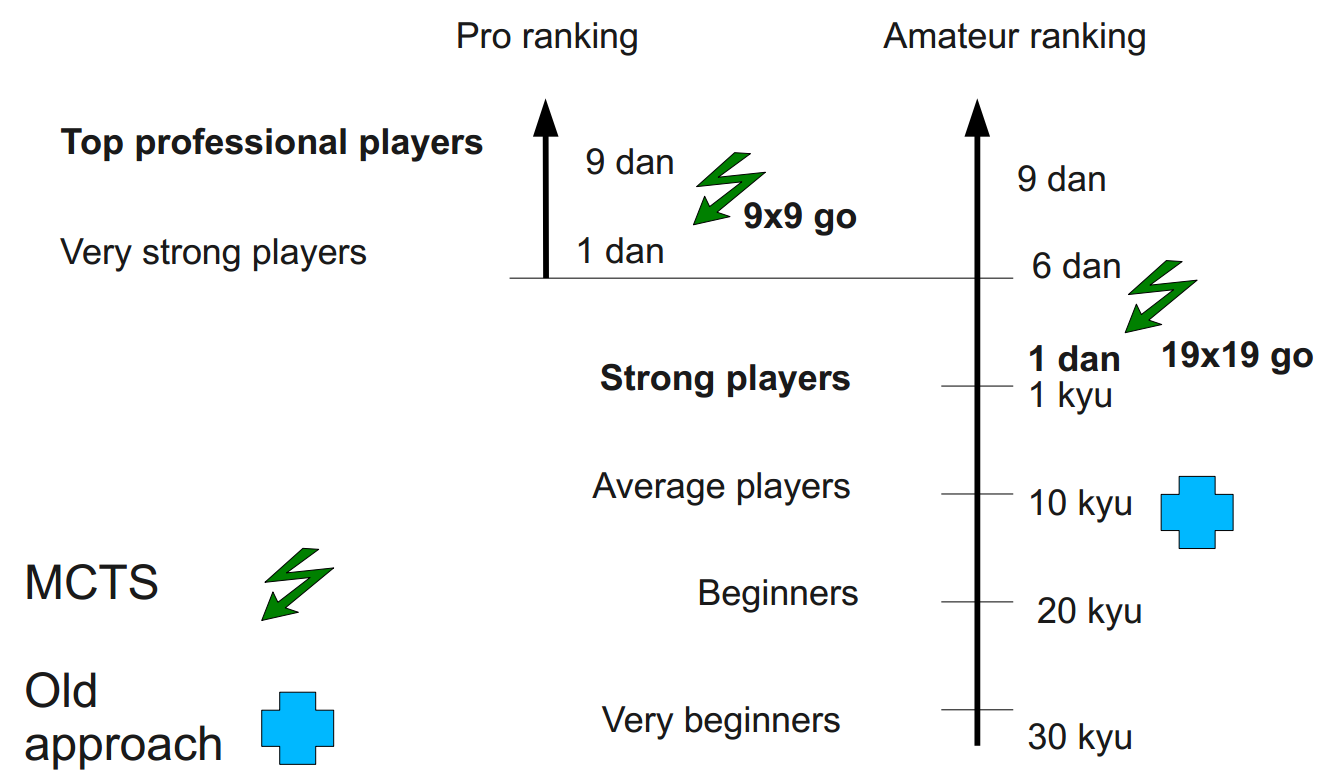
\includegraphics[width=12cm]{4_Strategies_and_state_of_the_art/4.8Arimaa_on_MCTS_Benoit/img/ranking.png}
\caption{\label{fig:ranking}Comparison between Go algorithms and human skill (\textit{2011})\cite{graphic_MCTS_Go}.}
\end{figure}
\textit{The ranking system of the game of Go is the following: kyu are for students' ranks, Dan are masters' ranks. Beginners start at 30 kyu and advance downward on the kyu grades system. Once a player ranks over 1 kyu, he will receive the 1st Dan (like the black belt in Judo) and will move upward through the Dan ranks until the 9th.}\bigskip
\\

For \emph{Arimaa}, the \emph{MCTS} algorithm was not the first method applied in order to solve it; the \ensuremath{\alpha\beta} method was used beforehand. At the moment the top programs (Bomb by David Fotland: 2002 to 2008, Clueless by Jeff Bacher 2009) are ranked about 1800 elo\footnote{\textit{The Elo rating system is a method for calculating the relative skill levels of players in competitor-versus-competitor games such as chess. It is also used for Arimaa. Beginners rank around 1200 elo, experts around 2000 elo and International Masters over 2400 elo.}}. For comparison, strongest humans players are rated around 2450 elo.\cite{master_mcts_kozeleck}
\medskip
